\newpage % Rozdziały zaczynamy od nowej strony.
\section{Charakterystyka projektów}
W celu lepszego zrozumienia roli kierownika projektu warto najpierw przedstawić i przypomnieć podstawowe informacje na temat projektów oraz zarządzania nimi. Rozdział ten pozwoli na ponowne spojrzenie na projekt w ramach teoretycznych, w oderwaniu od emocji związanych z doświadczeniami prywatnymi, które mogą wpływać na zrozumienie całości tematu. Oprócz podstawowej definicji projektu przytoczone zostaną szczegółowe statystyki dotyczące rosnącego znaczenia projektów oraz ich rezultatów.

\subsection{Definicja projektu}

Projekt to tymczasowe przedsięwzięcie podejmowane w celu stworzenia unikalnego produktu, usługi lub rezultatu. Tymczasowy charakter projektu oznacza określony początek i koniec. Koniec projektu następuje, gdy jego cele zostaną osiągnięte lub gdy projekt zostaje zakończony, ponieważ jego cele nie mogą zostać zrealizowane lub potrzeba projektu przestaje istnieć. Tymczasowość niekoniecznie oznacza krótki czas trwania. Tymczasowość zazwyczaj nie dotyczy produktu, usługi lub rezultatu stworzonego przez projekt; większość projektów jest podejmowana w celu osiągnięcia trwałego rezultatu. \autocite{pmbok}
Turner \autocite{Turner2016} zwraca szczególną uwagę w swojej definicji projektu na to, że projekt ma za zadanie dostarczyć unikatową zmianę. Zmiana ta może być rozumiana jako nowy produkt, np. budynek, ale również jako coś bardziej abstrakcyjnego i niematerialnego, np. nowa struktura organizacyjna w firmie. Turner podkreśla również, że zmiana ta powinna przynosić organizacji korzyści. Projekt nie może mieć na celu generowania strat, a w perspektywie długoterminowej powinien wpisywać się w cele strategiczne organizacji.
Według Turnera projekt nie jest jedynie wykonywaniem określonej pracy w ramach ustalonego czasu, kosztów i jakości. Ograniczenia te są istotą wszystkich działań, zarówno biznesowych, jak i prywatnych. Projekt definiują również złożoność i powtarzalność wymaganych prac. Charakterystyka projektu w porównaniu z procesami i funkcjami w organizacji została przedstawiona na rysunku 2.1. Projekt to działanie o dużej złożoności i niskiej powtarzalności, a warunki projektu są zawsze wyjątkowe, co wymaga dostosowania działań do konkretnych okoliczności.
\begin{figure}
\centering
\caption{Porównanie projektów i funkcji}
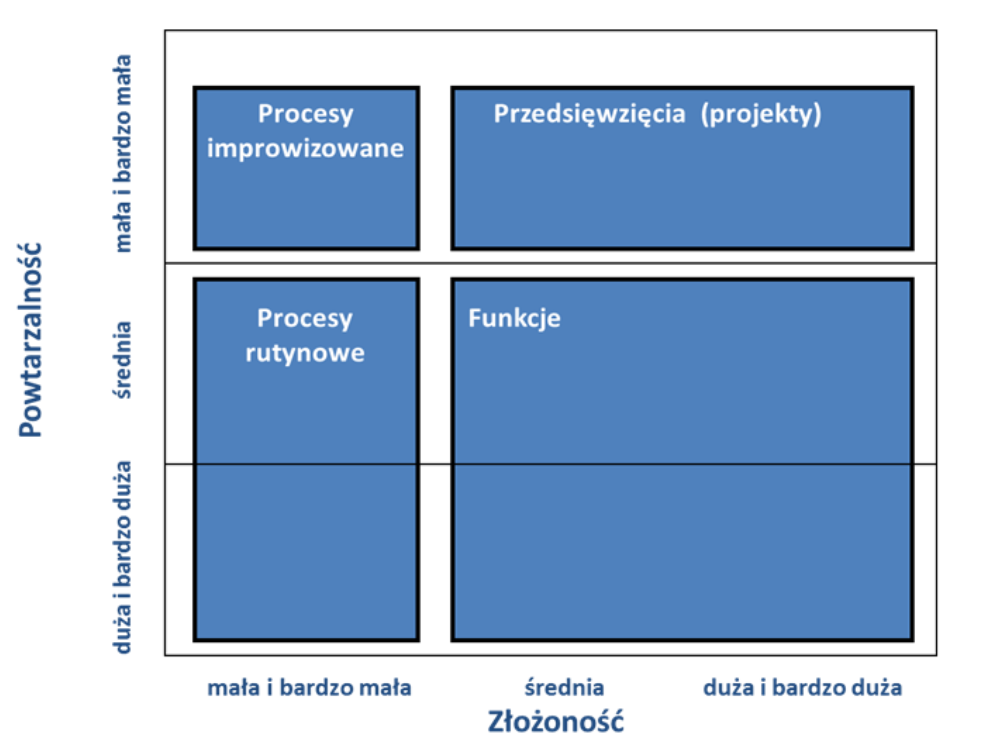
\includegraphics[width=14cm]{img/projekt.png}
\caption*{Źródło: M. Trocki, B. Grucza, K. Ogonek, \textit{Zarządzanie projektami}, PWE, Warszawa 2003, s. 14}
\end{figure}
Kerzner \autocite{Kerzner2017} oraz Turner \autocite{Turner2016} za istotę projektu uznają również to, że projekt wymaga integracji zarówno materialnych, jak i niematerialnych zasobów organizacji. Kerzner posługuje się grafiką, która została przedstawiona na rysunku 2.2. Przedstawia on zasoby organizacji jako samotne wyspy powstałe w wyniku podziału organizacji na piony funkcyjne oraz warstwy zarządcze. Wyspy te w ramach projektu łączone są w tymczasową organizację mającą wspólny cel. Jednak osiągnięcie współpracy między tymi samodzielnymi jednostkami nie jest łatwe, dlatego odpowiednia koordynacja staje się kluczowym elementem projektu. Turner natomiast w kontekście wykorzystania zasobów w projekcie podkreśla, że podział organizacji na mniejsze jednostki, czyli zespoły projektowe, otwiera przed nią nowe możliwości, które wcześniej były nieosiągalne. Autor porównuje tę sytuację do tankowca i floty małych jachtów. Gdy przed obiema jednostkami postawi się zadanie przewozu ropy, wykorzystanie tankowca będzie bardziej efektywne. Jednak tankowiec nie jest w stanie wykonywać ostrych zwrotów ani przepłynąć przez wszystkie śluzy. Zespoły projektowe pozwalają osiągnąć zwinność małych jachtów, która jest niezbędna w działaniach charakteryzujących się dużą niepewnością, takich jak projekty.
\begin{figure}
\centering
\caption{Struktura w organizacjach}
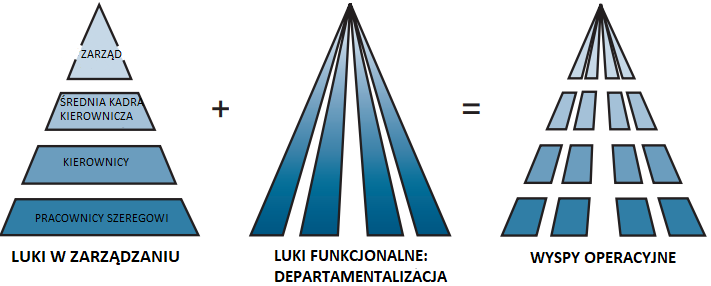
\includegraphics[width=15cm]{img/organizacja_PL.png}
\caption*{Źródło:  H. Kerzner. Project Management: A Systems Approach to Planning, Scheduling, and Controlling. John
Wiley \& Sons, 2017}
\end{figure}
\begin{figure}
\centering
\caption{Żelazny trójkąt projektu}
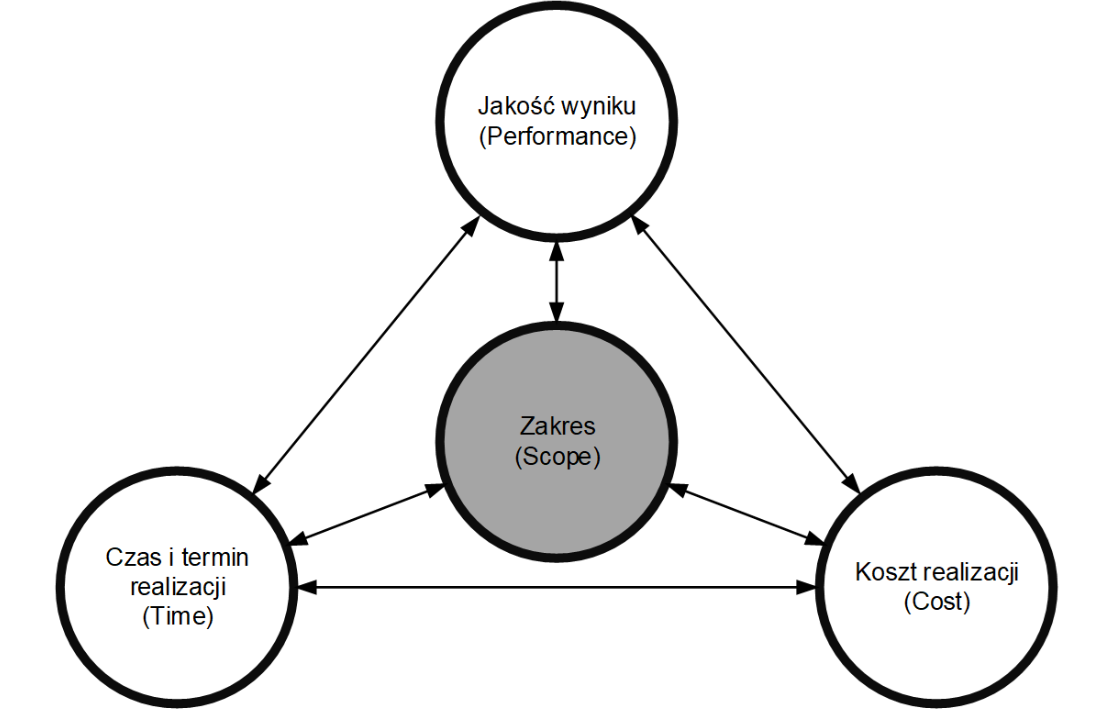
\includegraphics[width=14cm]{img/projekt2.png}
\caption*{Źródło: Wykład \textit{Podstawy Zarządzania Projektami}, Mateusz Juchniewicz}
\end{figure}

\subsection{Żelazny trójkąt projektu}
W celu ułatwienia zrozumienia kluczowych ograniczeń projektu opracowano koncepcję żelaznego trójkąta projektu. Ukazuje ona wzajemne zależności między czterema kluczowymi ograniczeniami projektu: zakresem, czasem, jakością i kosztem. \autocite{triangle} \autocite{challanges}
Zakres definiuje wszystkie prace niezbędne do stworzenia finalnego produktu, usługi lub rezultatu projektu. Obejmuje on cele, zadania, funkcje i cechy projektu. \autocite{triangle2}
Czas to okres trwania projektu, od początku do końca. Obejmuje harmonogram zadań, kamienie milowe i ostateczny termin zakończenia projektu.
Jakość odnosi się do stopnia, w jakim produkt, usługa lub rezultat projektu spełniają określone wymagania i standardy. Obejmuje zarówno aspekty funkcjonalne, jak i niefunkcjonalne, a także oczekiwania interesariuszy.
Koszt to całkowita kwota pieniędzy niezbędna do sfinansowania projektu. Uwzględnia on zasoby, materiały, wynagrodzenia, narzędzia i inne wydatki.
Główna idea trójkąta projektu polega na tym, że zmiana jednego z tych ograniczeń nieuchronnie wpływa na co najmniej jedno z pozostałych.
Na przykład:
\begin{itemize}
    \item Zwiększenie zakresu prac projektu zazwyczaj wymaga wydłużenia czasu trwania projektu lub zwiększenia budżetu.
    \item Skrócenie czasu realizacji projektu może wiązać się z koniecznością zwiększenia kosztów (np. poprzez zatrudnienie dodatkowych zasobów) lub obniżenia jakości.
    \item Podniesienie standardów jakości często wymaga więcej czasu i pieniędzy.
\end{itemize}
Trójkąt projektu jest jednak jedynie uproszczonym modelem, który nie uwzględnia wszystkich aspektów projektu. Nie uwzględnia on na przykład ryzyka, zasobów ludzkich, zarządzania zakłóceniami czy satysfakcji klienta. Należy o tym pamiętać, interpretując wyniki analizy opartej na tym modelu.
Mimo to trójkąt projektu pozostaje cennym narzędziem w zarządzaniu projektami. Pomaga on lepiej zrozumieć podstawowe zależności między zakresem, czasem, jakością i kosztem. Trójkąt projektu wspiera również komunikację tych zależności interesariuszom projektu oraz pozwala na podejmowanie bardziej świadomych decyzji dotyczących kompromisów i alokacji zasobów.

\subsection{Projektyzacja}
W ostatnich latach rosnące znaczenie projektów w działalności organizacji zaowocowało pojawieniem się zjawiska projektyzacji, które polega na zastępowaniu tradycyjnych, powtarzalnych działań unikatowymi przedsięwzięciami realizowanymi jako projekty \autocite{Juchniewicz2018}. Proces ten wpływa zarówno na struktury organizacyjne, jak i na podejście do zarządzania w sektorach publicznym i prywatnym \autocite{Midler1995}.
Pojęcie projektyzacji zostało wprowadzone już w latach 90. XX wieku. Kluczowe badania przeprowadzone przez Midlera oraz Maylora i współpracowników \autocite{Maylor2006} wskazują, że transformacja organizacyjna polega nie tylko na zwiększeniu liczby realizowanych projektów, ale przede wszystkim na zmianie sposobu, w jaki organizacje planują i wdrażają swoje działania. Proces projektyzacji niesie ze sobą zarówno korzyści, jak i pewne zagrożenia. Z jednej strony umożliwia on zwiększenie elastyczności organizacyjnej i szybką reakcję na zmieniające się warunki rynkowe \autocite{Prawelska2011}. Z drugiej strony jednak, ciągła intensyfikacja realizowanych projektów może prowadzić do nadmiernego obciążenia pracowników, wzrostu presji i stresu, a także do fragmentacji działań organizacyjnych \autocite{Jalocha2012}.
\\
Aktualne dane statystyczne pokazują, że projekty stanowią coraz większy udział w działalności organizacji. PriceWaterhouseCoopers w swoim raporcie podaje, że globalne wydatki na publiczne projekty inwestycyjne wzrosną z poziomu 4 bln USD w 2012 r. do ok. 9 bln USD w 2025 r. \autocite{pwc}
Dodatkowo A. Nieto-Rodriguez stwierdza, że udział projektów jako źródła globalnego produktu brutto będzie ciągle rósł. Szacuje się,
że do ok. 2025 r. wyniesie on ok. 35\% \autocite{Nieto}. Rysunek 2.4 przedstawia szacunkowe dane obrazujące to zjawisko.
\begin{figure}
\centering
\caption{Stosunek projektów do operacji w organizacjach}
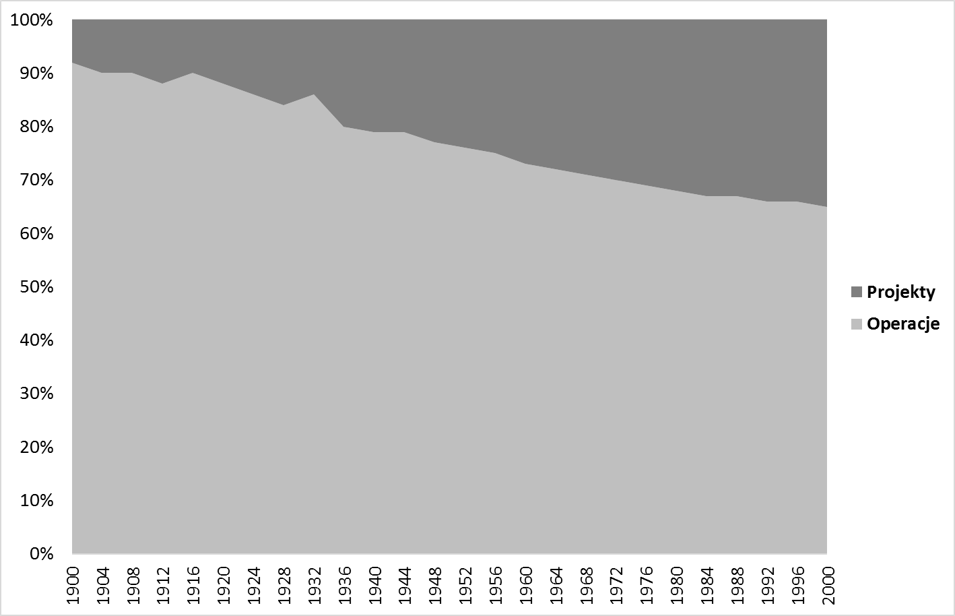
\includegraphics[width=14cm]{img/projektyzacja.png}
\caption*{Źródło: Wykład \textit{Podstawy Zarządzania Projektami}, M. Juchniewicz}
\end{figure}
Potwierdzeniem rosnącego znaczenia projektów są również raporty PMI, w których zauważono znaczący wzrost liczby biur projektów w organizacjach. Rysunek 2.5 przedstawia wspomniane statystyki. Według tego raportu odsetek organizacji posiadających biuro projektowe wzrósł z 61\% w 2007 r. do 70\% w 2017 r.
\begin{figure}
\caption{Procent organizacji z biurem zarządzania projektami}
\centering
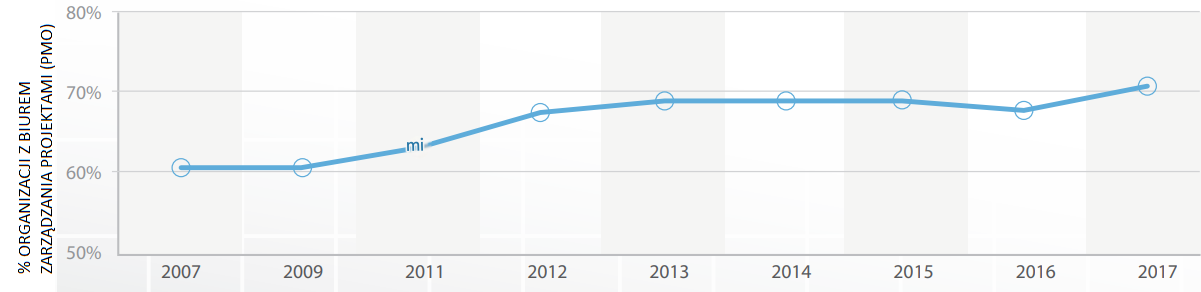
\includegraphics[width=15cm]{img/pmos_PL.png}
\caption*{Źródło: \textit{Pulse of the Profession}, PMI 2017}
\end{figure}
PMI podał również, że liczba stanowisk związanych z zarządzaniem projektami osiągnęła w 2017 roku prawie 66 milionów, a popyt wciąż rośnie. „Do 2027 roku pracodawcy będą potrzebować 87,7 miliona osób na stanowiskach związanych z zarządzaniem projektami.” \autocite{job}

Kolejnym przykładem projektyzacji może być polski sektor publiczny, w którym projekty w wielu organizacjach stanowią już około 60-80\% wszystkich działań \autocite{Prawelska2011}.

\subsection{Rezultaty projektów}
Warte wspomnienia są również statystyki dotyczące rezultatów realizowanych projektów. Według raportu PMI jedynie 70\% projektów osiąga pierwotnie założone cele, a około 15\% jest uznawanych za całkowitą porażkę. Rysunek 2.6 przedstawia te statystyki w sposób bardziej szczegółowy.
\begin{figure}
\centering
\caption{Rezultaty projektów}
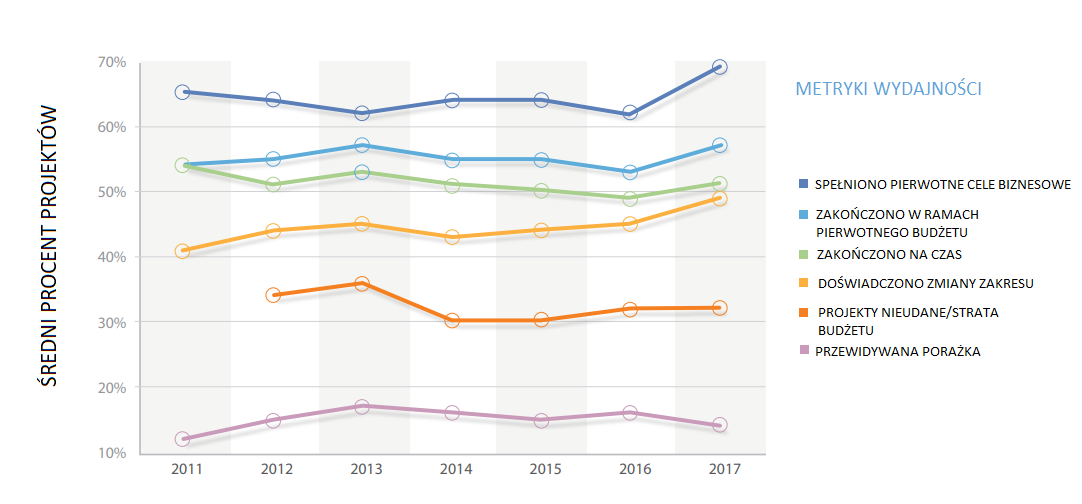
\includegraphics[width=16cm]{img/pmi_rezultaty_PL.png}
\caption*{Źródło: \textit{Pulse of the Profession}, PMI 2017}
\end{figure}
Raport Arras People jest jeszcze bardziej pesymistyczny – aż 41\% respondentów zgłasza, że projekty, w których uczestniczyli, zakończyły się porażką. \autocite{arras2010}
Takie dane sugerują, że mimo rosnącej liczby realizowanych projektów, wiele z nich nie przynosi oczekiwanych rezultatów, co stanowi istotne wyzwanie dla współczesnych organizacji.

\subsection{Projekty informatyczne w kontekście rosnącej liczby projektów}
Projekty informatyczne stanowią istotny segment realizowanych przedsięwzięć, zwłaszcza w kontekście cyfryzacji i dynamicznych zmian technologicznych. Według Gartner światowe wydatki na IT wyniosły 3,5 biliona dolarów w 2017 roku, co oznacza wzrost o 2,4\% w porównaniu z rokiem 2016.\autocite{gartner} Mimo rosnącej liczby projektów informatycznych, wyniki ich realizacji często pozostawiają wiele do życzenia i wypadają one znacznie gorzej na tle innych typów przedsięwzięć. Według raportu Standish Group jedynie 30\% projektów informatycznych osiąga pełne cele, natomiast 50\% wykazuje problemy operacyjne, takie jak opóźnienia czy przekroczenia budżetowe. Aż 20\% analizowanych projektów informatycznych zakończyło się porażką 
\begin{table}[h]
    \caption{Rezultaty projektów w latach 2011-2015}
    \label{tab:projekty}
    \centering
    \renewcommand{\arraystretch}{1.5}
    \setlength{\tabcolsep}{10pt}
    \rowcolors{2}{white}{yellow!20}
    \begin{tabular}{|l|c|c|c|c|c|}
        \hline
        \rowcolor{blue!50} 
        \multicolumn{1}{|c|}{} & \textbf{2011} & \textbf{2012} & \textbf{2013} & \textbf{2014} & \textbf{2015} \\
        \hline
        \rowcolor{green!50} \textbf{Sukces} & 29\% & 27\% & 31\% & 28\% & 29\% \\
        \hline
        \rowcolor{yellow!50}
        \textbf{Wyzwania} & 49\% & 56\% & 50\% & 55\% & 52\% \\
        \hline
        \rowcolor{red!50} \textbf{Niepowodzenie} & 22\% & 17\% & 19\% & 17\% & 19\% \\
        \hline
    \end{tabular}
    \caption*{Źródło: \textit{CHAOS Report}, Standish Group 2015}
\end{table}


\begin{table}[ht]
\centering
\caption{Podsumowanie wyników badania CHAOS}
\label{tab:chaos_summary}
\begin{tabular}{lccc}
\toprule
& \textbf{Duże} & \textbf{Średnie} & \textbf{Małe} \\
\midrule
\textbf{Średni koszt rozwoju} & \$2{,}322{,}000 & \$1{,}331{,}000 & \$434{,}000 \\
\textbf{Średnie przekroczenie kosztów} & 189\% & 178\% & 112\% \\
\textbf{Średnie przekroczenie harmonogramu} & 222\% & 220\% & 239\% \\
\textbf{Zachowane oryginalne funkcje} & 42\% & 65\% & 74\% \\
\textbf{Projekty zakończone sukcesem} & 9.6\% & 16.2\% & 28.0\% \\
\textbf{Projekty z wyzwaniami} & 61.5\% & 46.7\% & 46.7\% \\
\textbf{Projekty nieudane} & 29.5\% & 37.1\% & 25.3\% \\
\bottomrule
\end{tabular}
\caption*{Źródło: \textit{CHAOS Report}, Standish Group 2015}

\end{table}

Podobne dane raportuje również World Bank Group. Według ich statystyk jedynie 13\% projektów informatycznych z sektora dużych przedsiębiorstw kończy się sukcesem. Dodatkowo przedstawili oni porównanie projektów informatycznych do wszystkich projektów, z którego wynika, że te związane z teleinformatyką wyraźnie odnotowują gorsze rezultaty. Obie te statystyki zostały przedstawione na rysunkach 2.7. i 2.8. Według ankiety przeprowadzonej wśród specjalistów i kadry kierowniczej z branży technologicznej, zarówno w sektorze publicznym, jak i prywatnym, powodem wysokiego odsetka niepowodzeń projektów informatycznych jest słabe zaangażowanie użytkowników, brak wsparcia kierownictwa oraz nieprecyzyjne określenie wymagań projektu \autocite{wdr}.

\begin{figure}[htbp]
\centering
\caption{Wskaźnik sukcesu dużych projektów informatycznych w sektorze publicznym}
\begin{tikzpicture}
\pie[text=legend, sum=100, color={red!70, orange!70, green!70}, radius=3]{
    58/Sukces,
    29/Częściowe niepowodzenie,
    13/Niepowodzenie
}
\end{tikzpicture}

\label{fig:B3.5.1}

\caption*{Źródło: \textit{World Development Report}, World Bank Group 2016}
\end{figure}


\begin{figure}
\centering
\caption{Porównanie sukcesu dla projektów informatycznych i wszystkich projektów}
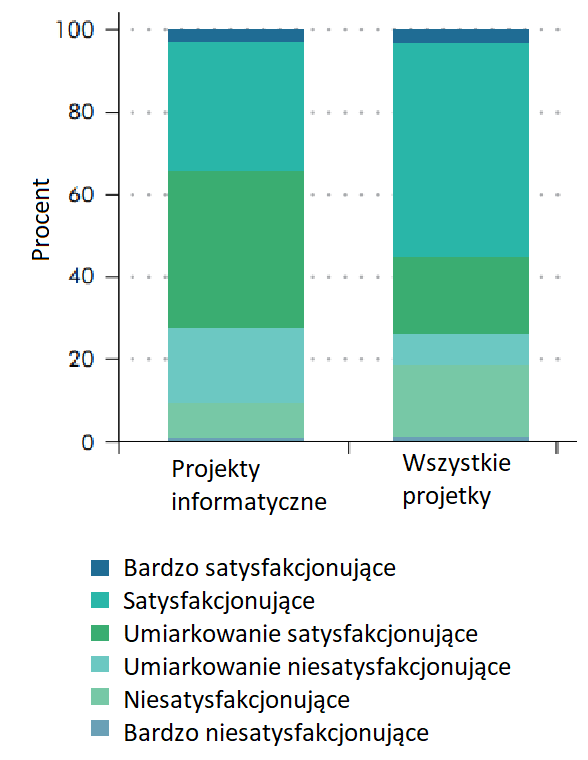
\includegraphics[width=9cm]{img/wdr2_PL.png}
\caption*{Źródło: \textit{World Development Report}, World Bank Group 2016}
\end{figure}